\documentclass[notheorems,mathserif,table,compress]{beamer}  %dvipdfm选项是关键,否则编译统统通不过
%%------------------------常用宏包------------------------
%%注意, beamer 会默认使用下列宏包: amsthm, graphicx, hyperref, color, xcolor, 等等
\usepackage{fontspec,xunicode,xltxtra}  % for XeTeX
\usepackage{comment}
\usepackage{fancybox}
 \usepackage{enumerate}
\usepackage{color}

%%------------------------ThemeColorFont------------------------
%% Presentation Themes
% \usetheme[<options>]{<name list>}
\usetheme{Madrid}
%% Inner Themes
% \useinnertheme[<options>]{<name>}
%% Outer Themes
% \useoutertheme[<options>]{<name>}
\useoutertheme{miniframes} 
%% Color Themes 
% \usecolortheme[<options>]{<name list>}
%% Font Themes
% \usefonttheme[<options>]{<name>}
\setbeamertemplate{background canvas}[vertical shading][bottom=white,top=structure.fg!7] %%背景色, 上25%的蓝, 过渡到下白.
\setbeamertemplate{theorems}[numbered]
\setbeamertemplate{navigation symbols}{}   %% 去掉页面下方默认的导航条.
\usepackage{zhfontcfg}
\usepackage{wrapfig}
%\setsansfont[Mapping=tex-text]{文泉驿正黑}  %% 需要fontspec宏包
     %如果装了Adobe Acrobat,可在font.conf中配置Adobe字体的路径以使用其中文字体
     %也可直接使用系统中的中文字体如SimSun,SimHei,微软雅黑 等
     %原来beamer用的字体是sans family;注意Mapping的大小写,不能写错
     %设置字体时也可以直接用字体名,以下三种方式等同:
     %\setromanfont[BoldFont={黑体}]{宋体}
     %\setromanfont[BoldFont={SimHei}]{SimSun}
     %\setromanfont[BoldFont={"[simhei.ttf]"}]{"[simsun.ttc]"}
%%------------------------MISC------------------------
\graphicspath{{figures/}}         %% 图片路径. 本文的图片都放在这个文件夹里了.
%%------------------------正文------------------------
\begin{document}
\XeTeXlinebreaklocale "zh"         % 表示用中文的断行
\XeTeXlinebreakskip = 0pt plus 1pt % 多一点调整的空间
%%----------------------------------------------------------
%% This is only inserted into the PDF information catalog. Can be left
%% out.
%%%
%% Delete this, if you do not want the table of contents to pop up at
%% the beginning of each subsection:
\begin{comment}
\AtBeginSection[]{                              % 在每个Section前都会加入的Frame
  \frame<handout:0>{
    \frametitle{Content}\small
    \tableofcontents[current,currentsubsection]
  }
}
\AtBeginSubsection[]                            % 在每个子段落之前
{
  \frame<handout:0>                             % handout:0 表示只在手稿中出现
  {
    \frametitle{下一节内容}\small
    \tableofcontents[current,currentsubsection] % 显示在目录中加亮的当前章节
  }
}
\end{comment}
%%----------------------------------------------------------
\title[Region-based Segmentation]{Region-based Segmentation}
\subtitle{基于区域的图像分割}
\author[赵海伟\ 王如晨\ 戴嘉伦]{\textcolor{olive}{赵海伟\ 王如晨\ 戴嘉伦}}
  %\hspace{2.28em}导师~~\textcolor{olive}{姬光荣}~教授}
\institute[CVBIOUC]{\small\textcolor{violet}{CVBIOUC}}
\date{\today}
%\titlegraphic{\vspace{-6em}\includegraphics[height=7cm]{ouc}\vspace{-6em}}
\frame{ \titlepage }
%%----------------------------------------------------------
%\section*{目录}
%\frame{\frametitle{目录}\tableofcontents}
%%----------------------------------------------------------

%\section{Beamer类和XeTeX概览} %如果你想书签不出现问题,请不要用\XeTeX
                                 %这类复杂的指令,直接写XeTeX吧

\begin{comment}
\section{Image Segmentation}
\subsection{Introduction}
\begin{frame}
    \frametitle{Introduction}
    \textbf{Image segmentation:} 
	\begin{itemize}
	\item The process of partitioning a digital image into \textbf{multiple segments}.\newline
	\end{itemize}
    \textbf{The goal of segmentation:}
	\begin{itemize}
	\item \textbf{Simplify} and \textbf{change} the representation of an image into something that is more meaningful and easier to analyze 
	\end{itemize}
\end{frame}


\begin{frame}
    \frametitle{Introduction}
   \begin{figure}
   \begin{minipage}[t]{0.4\textwidth}
   \centering
   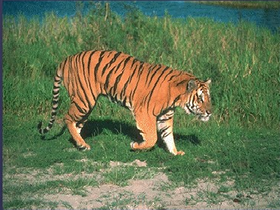
\includegraphics[width=1.8in]{tiger1.png}
   \end{minipage}
   \begin{minipage}[t]{0.4\textwidth}
   \centering
   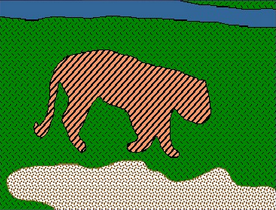
\includegraphics[width=1.8in]{tiger2.png}
   \end{minipage} 
   \end{figure}
\end{frame}

\begin{frame}
\frametitle{Introduction}
   \begin{figure}[!ht]
   \begin{minipage}[t]{0.4\textwidth}
   \centering
   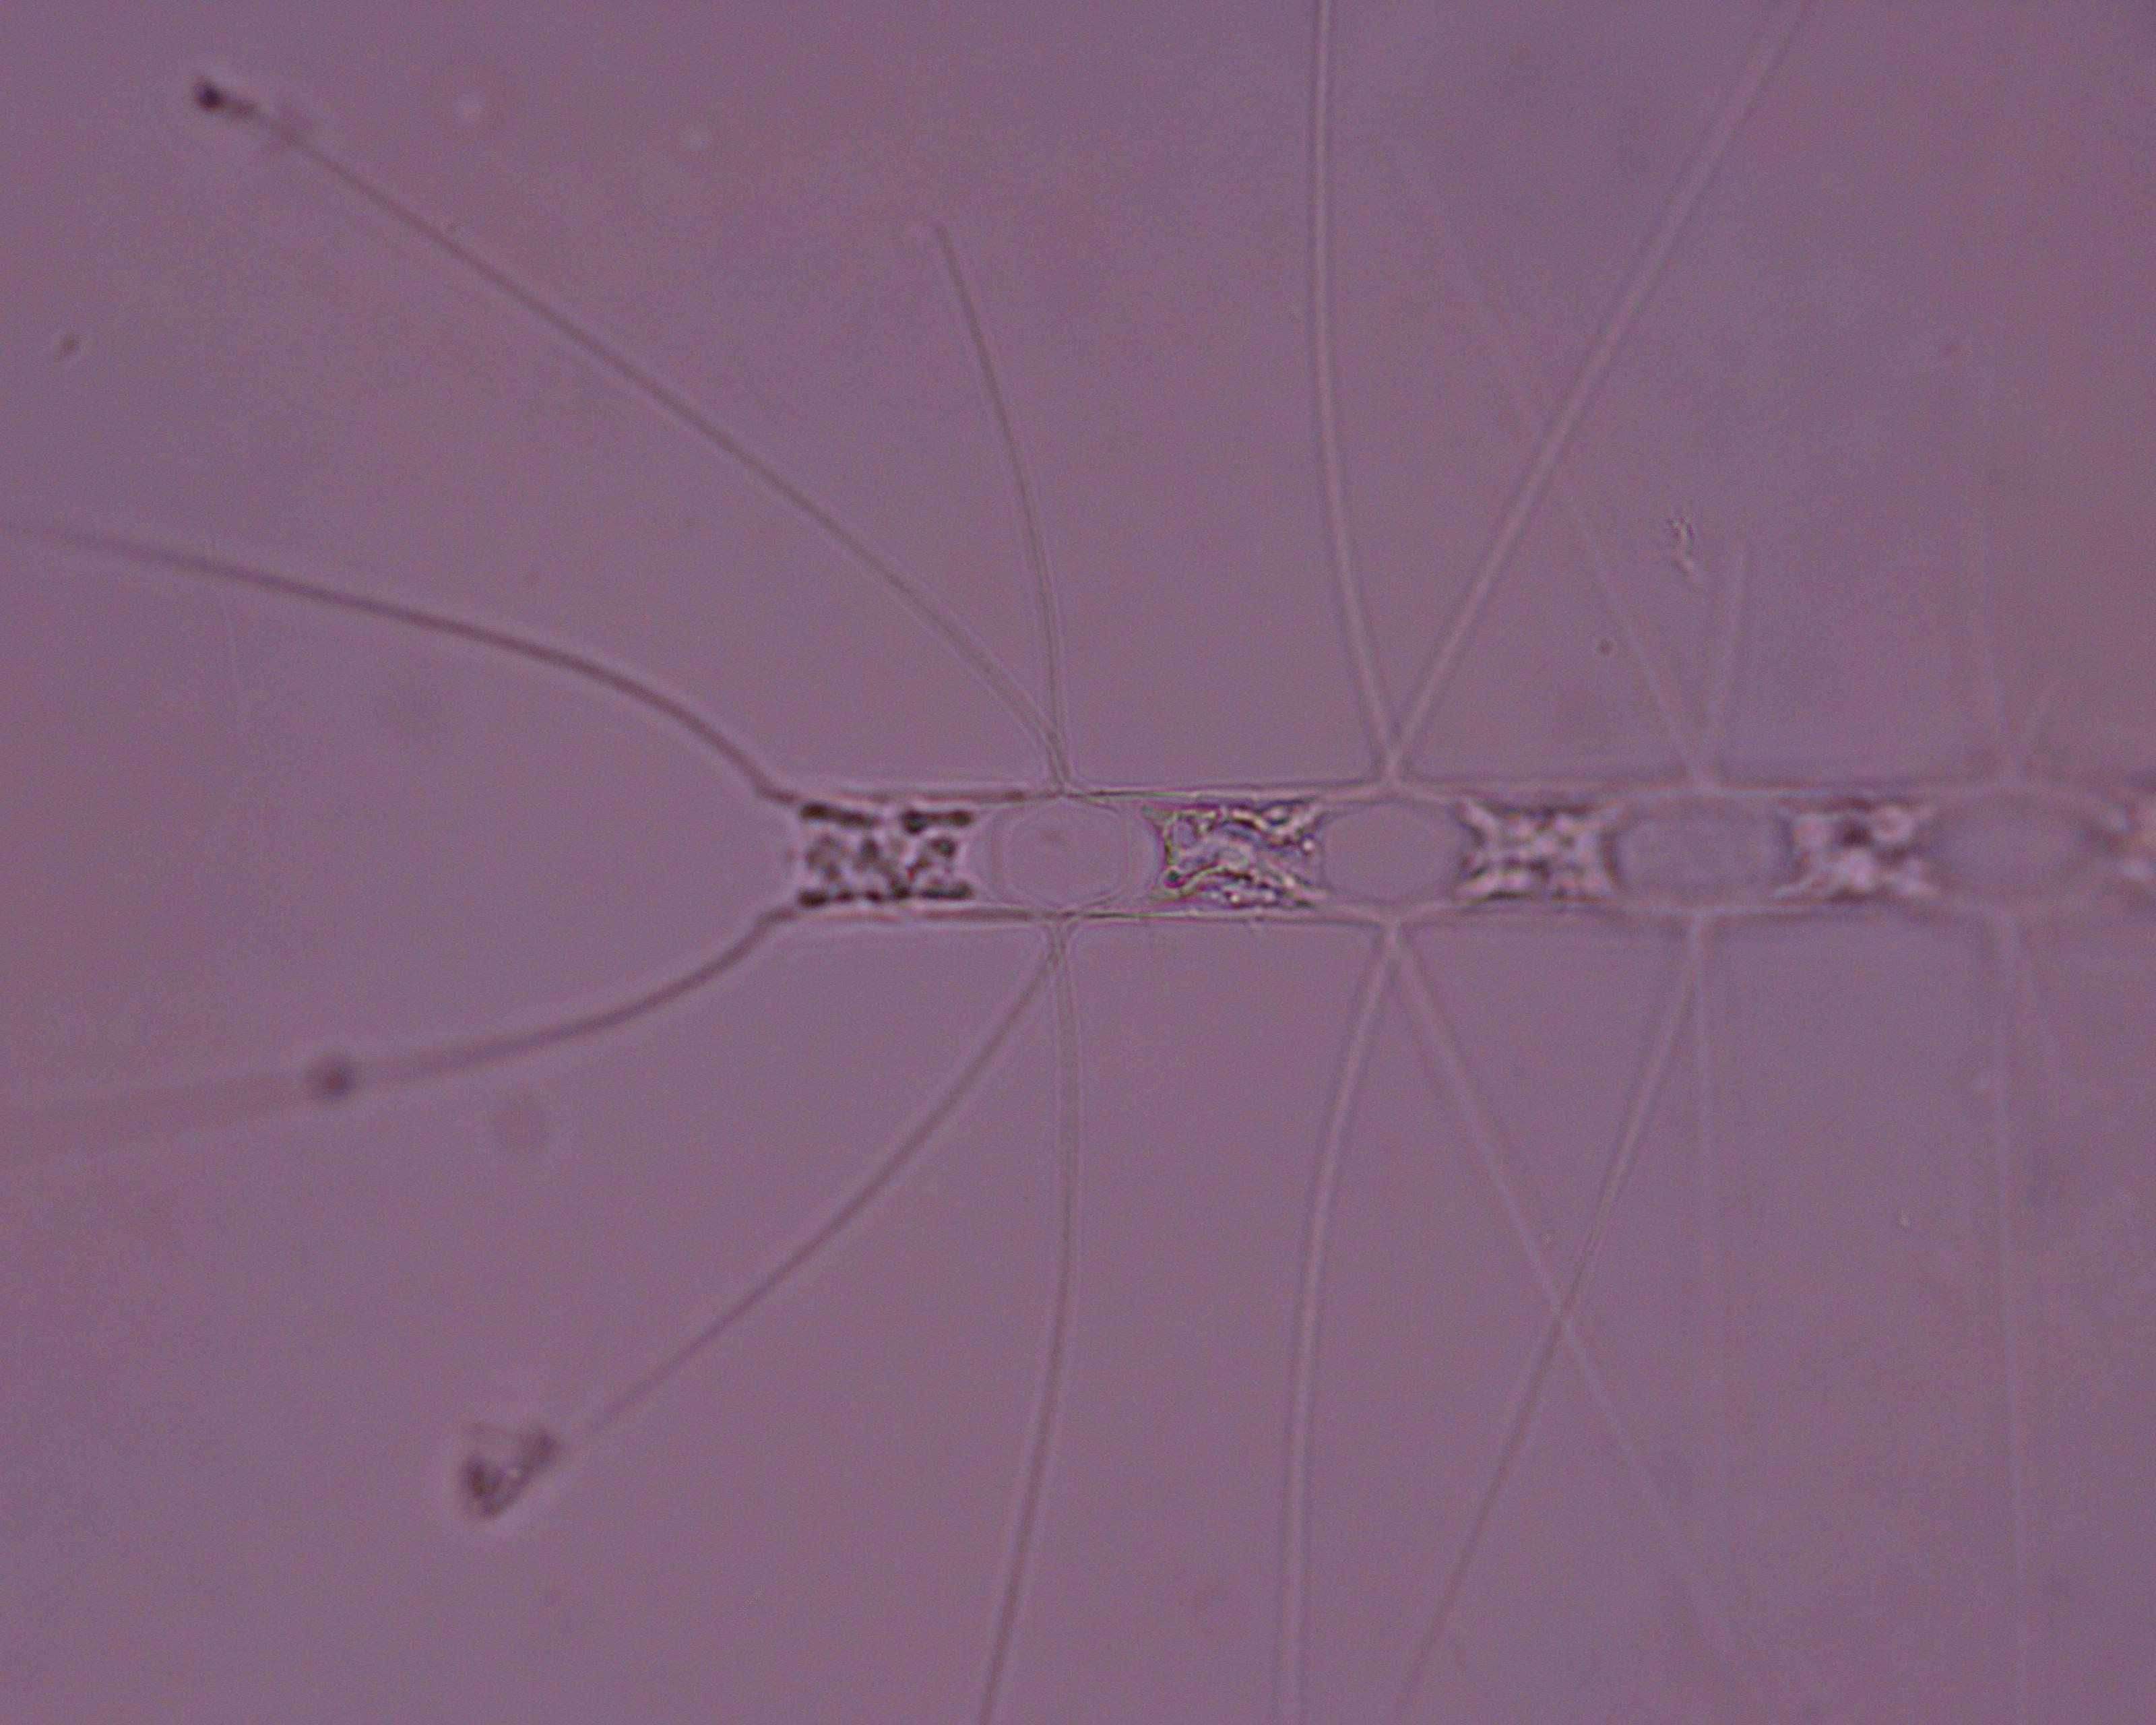
\includegraphics[width=1.8in]{algea.jpg}
   \end{minipage}
   \begin{minipage}[t]{0.4\textwidth}
   \centering
   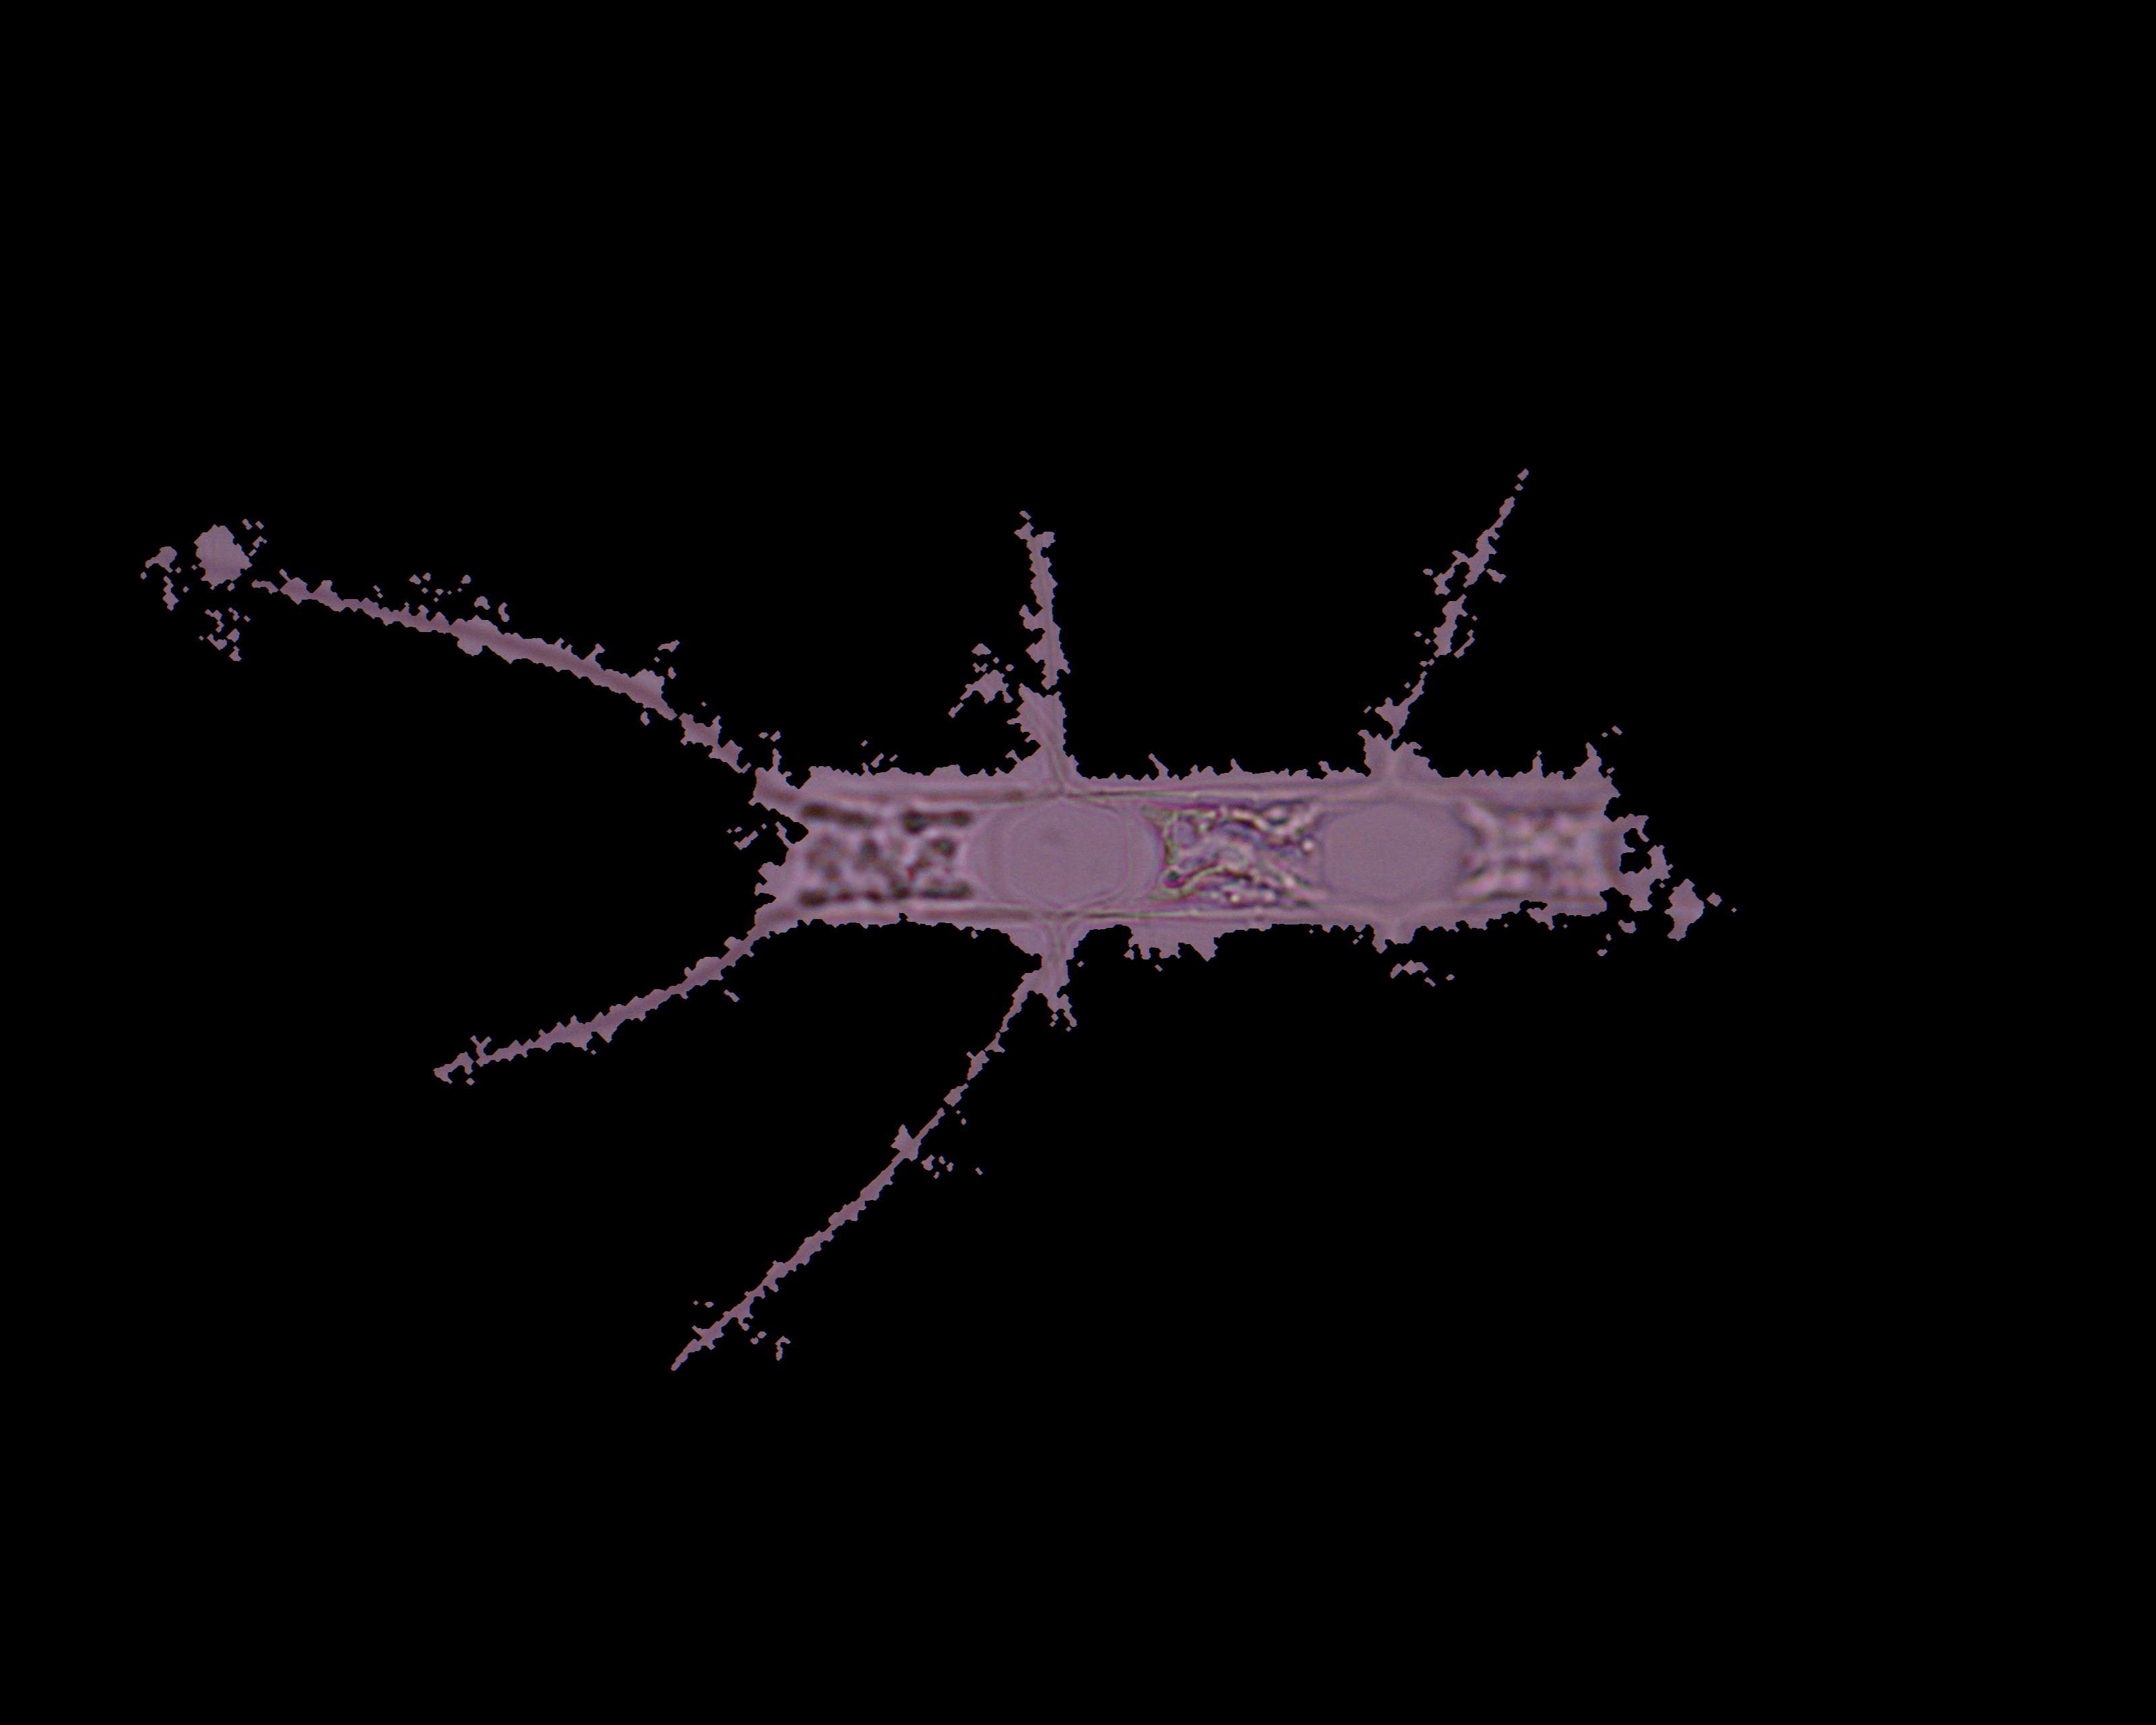
\includegraphics[width=1.8in]{algea2.jpg}
   \end{minipage} 
   \end{figure} 
\end{frame}

\begin{frame}
    \frametitle{Introduction}
    %Pre-process $\Longrightarrow$ Object Detection $\Longrightarrow$ Image Segmentation $\Longrightarrow$ Image Recognition
    \begin{figure}[!ht]
    \centering
    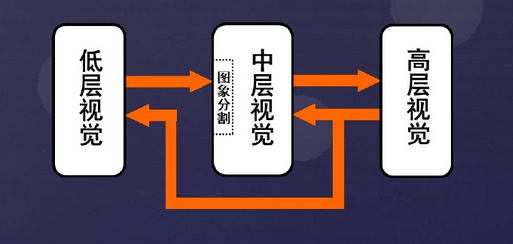
\includegraphics[width=3.0in]{path.png}
    \end{figure} 
\end{frame}




\subsection{Methods}
\begin{frame}
    \frametitle{Methods}
    \begin{itemize}
    \item Thresholding
    \item Edge-based Segmentation
    \item Region-based Segmentation
    \item State-of-the-art Methods
    \end{itemize}
   % Choice of technique depends on peculiar characteristics of individual problems.//
 %   A universal algorithm of segmentation does not exist, as each type of image corresponds to a specific approach
\end{frame}

\begin{frame}
    \frametitle{Methods}
    Segmentation algorithms are generally based on \underline{\textbf{two basic properties}} of gray-scale values
    \begin{itemize}
    \item Discontinuity
    \item Similarity \newline
    \end{itemize}
   % \emph{\textbf{Choice of technique depends on peculiar characteristics of individual problems.}}\\
   %\definecolor{cyanlight}{rgb}{0.0, 0.72, 0.92}
   %\color{cyanlight}{text}
    {\color{blue}{\emph{\textbf{A universal algorithm of segmentation does not exist, as each type of image corresponds to a specific approach.}}}}
         %\emph{\textbf{A universal algorithm of segmentation does not exist, as each type of image corresponds to a specific approach}}

\end{frame}
\end{comment}



\section{Region-based Methods}
\begin{frame}
    \frametitle{Region-based Methods}
    \begin{enumerate}
    \item \textbf{\Large Region} \newline
    \item \textbf{\Large Region Growing}\newline
    \item \textbf{\Large Region Splitting and Merging} \newline
    \item \textbf{\Large Watershed} \newline
    \end{enumerate}
\end{frame}

\subsection{Region}
\begin{frame}
    \frametitle{Region}
%    \begin{itemize}
     \begin{columns}
     \begin{column}[c]{0.45\textwidth}
     \textbf{\Large Definition:}
        \begin{itemize}
	  \item[-] A group of connected pixels with \textbf{similar properties} \newline
         \end{itemize}
    \textbf{\Large Idea:}
          \begin{enumerate}
          \item[-] Similarity
          \item[-] Spatial Proximity
	 \end{enumerate}
    \end{column}

    \begin{column}[c]{0.55\textwidth}
    \begin{figure}[!ht]
    \begin{minipage}[t]{0.5\linewidth}
    \centering
    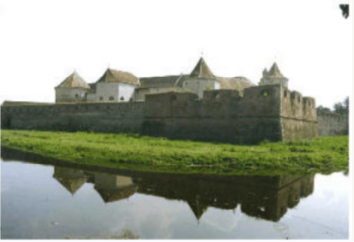
\includegraphics[width=1.8in]{region_1.png}
    \end{minipage}
    \begin{minipage}[t]{0.5\linewidth}
    \centering
    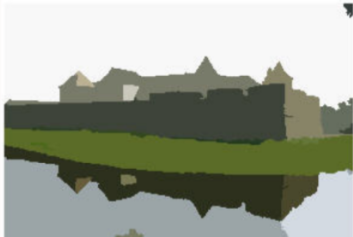
\includegraphics[width=1.8in]{region_2.png}
    \end{minipage}
    \end{figure}
    \end{column}
    \end{columns}
\end{frame}


\subsection{Region Growing}
\begin{frame}
    \frametitle{Region Growing}
    \begin{enumerate}[{\color{black}{\Large (A)}}]
    \item \textbf{\Large Idea:}
    \end{enumerate}
    	\begin{itemize}
    	\item[-] {\color{blue}{Seed}}: The regions are growing from seeds points.\\ \hspace{0.4in}The corresponding regions grow by appending those neighboring pixels to each seed points.
	\item[-] {\color{blue}{Pre-defined Criterion}}: It groups pixels or sub-regions into larger regions based on pre-defined criterion.
	\item[-] {\color{blue}{End Condition}}: The regions keep growing until meeting the end condition.
    	\end{itemize}
  \begin{figure}[!ht]
  \centering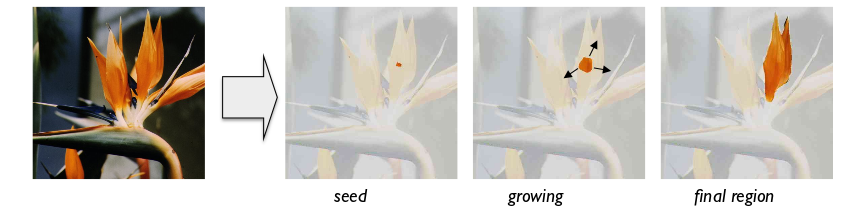
\includegraphics[width=4.0in]{region1.png}
  \end{figure} 
\end{frame}

\begin{comment}
\begin{frame}
    \frametitle{Region Growing}
  %  \begin{enumerate}[{\color{black}{\Large (A)}}]
     \textbf{\Large How do we choose the seeds}\\
     \begin{itemize}
     \item[-] It depends on the nature of the problem. 
     \item[-] {\emph{e.g.}} 
	\begin{itemize}
        \item[-] choose the brightest pixel in the image as seed point.
        \item[-]compute the histogram and choose the gray-level values corresponding to the strongest peaks
	\end{itemize}
     \end{itemize}
     \textbf{\Large How do we choose the similarity criterion}
  %  \end{enumerate}
  %  	\begin{itemize}
   % 	\item[-] {\color{blue}{Seed}}: The regions are grown from seeds points.\\ \hspace{0.4in}The corresponding regions grow by appending to each seed points those neighboring pixels.
%	\item[-] {\color{blue}{Pre-defined Criterion}}: It groups pixels or sub-regions into larger regions based on pre-defined criterion.
%	\item[-] {\color{blue}{End Condition}}: The regions keep growing until meeting the end condition.
  %  	\end{itemize}
\end{frame}
\end{comment}

\begin{comment}
\begin{frame}
    \frametitle{Region Growing}
    \begin{itemize}
    \item 区域生长的基本思想是将具有相似性质的像素集合起来构成区域
    \item 具体先对每个需要分割的区域找一个种子像素作为生长起点,然后将种子像素和周围邻域中与种子像素有相同或相似性质的像素(根据某种事先确定的生长或相似准则来判定),合并到种子像素所在的区域中。 
    \item 将这些新像素当作新的种子继续上面的过程,直到没有满足条件的像素可被包括进来。这样一个区域就生长成了。
    \end{itemize}
\end{frame}
\end{comment}

\begin{comment}
\begin{frame}
    \frametitle{Region Growing}
    \begin{itemize}
    \item 对图像顺序扫描!找到第1个还没有归属的像素, 设该像素为(x0, y0);
    \item 以(x0, y0)为中心, 考虑(x0, y0)的4邻域像素(x, y)如果(x0, y0)满足生长准则, 将(x, y)与(x0, y0)合并(在同一区域内), 同时将(x, y)压入堆栈
    \item 从堆栈中取出一个像素, 把它当作(x0, y0)返回到步骤2;
    \item 当堆栈为空时!返回到步骤1;
    \item 重复步骤1 – 4直到图像中的每个点都有归属时。生长结束。	
    \end{itemize}
\end{frame}
\end{comment}

\begin{frame}
    \frametitle{Region Growing}
    \begin{enumerate}[{\color{black}{\Large (B)}}]
    \item  \textbf{\Large Algorithm:}
    \end{enumerate}
  %  \textbf{\Large Algorithm:}
    \begin{itemize}
    \item[step1] Initially, the region $R$ needs to be extracted. The region $R$ only contains its seed point $p.$
    \item[step2] Initially, a queue $Q$ contains the boundary points of $R.$ $Q$ contains the 8-neighborhood or 4-neighborhood of the seed point $p$.
    \item[step3] While $Q$ is not empty:
    	\begin{itemize}
	\item[-] for each neighboring pixel $p*$ of $p$ in $Q:$
	     \begin{itemize}
	     \item[-] \emph{if}  $p*$ is similar to $p:$\\
	        \hspace{0.1in} {\color{blue}{-}} \hspace{0.05in} $p*$ is added to $R,$ $p*$ is marked with a label.\\
        	\hspace{0.1in} {\color{blue}{-}} \hspace{0.05in} neighboring pixels of $p*$ (not in $R$) are added to $Q.$
	     \item[-] \emph{else} set $p*$ as non-similar.
	     \end{itemize}
	\end{itemize}
 %   \item 以(x0, y0)为中心, 考虑(x0, y0)的4邻域像素(x, y)如果(x0, y0)满足生长准则, 将(x, y)与(x0, y0)合并(在同一区域内), 同时将(x, y)压入堆栈
 %   \item 从堆栈中取出一个像素, 把它当作(x0, y0)返回到步骤2;
 %   \item 当堆栈为空时!返回到步骤1;
 %   \item 重复步骤1 – 4直到图像中的每个点都有归属时。生长结束。	
    \end{itemize}
\end{frame}

\begin{frame}
  \frametitle{Region Growing}
  \begin{figure}[!ht]
  \centering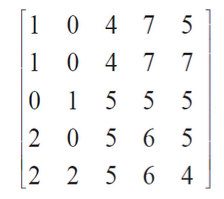
\includegraphics[width=1.5in]{grow_algorithm.png}
  \end{figure} 
\end{frame}

\begin{frame}
\frametitle{Region Growing}
\begin{figure}[!ht]
  \begin{minipage}[t]{0.3\textwidth}
  \centering
  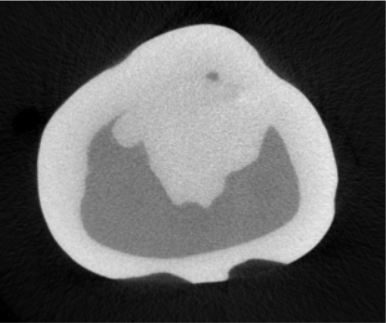
\includegraphics[width=1.4in]{seed1.png}
  \end{minipage}
  \begin{minipage}[t]{0.3\textwidth}
  \centering
  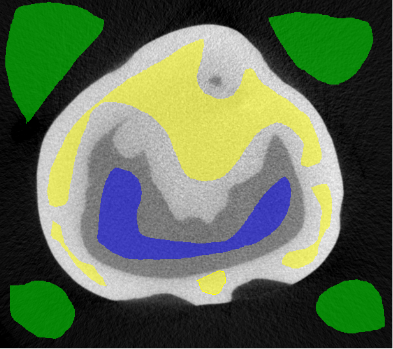
\includegraphics[width=1.3in]{seed2.png}
  \end{minipage}  
  \begin{minipage}[t]{0.3\textwidth}
  \centering
  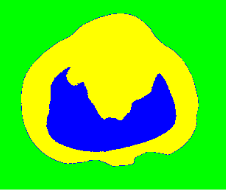
\includegraphics[width=1.4in]{seed3.png}
  \end{minipage}  
\end{figure} 
\end{frame}

\begin{frame}
    \frametitle{Region Growing}
    \begin{enumerate}[{\color{black}{\Large (C)}}]
    \item  \textbf{\Large Advantages:}
    \end{enumerate}
 %   \textbf{\Large Advantages:}\\
        \begin{itemize}
        \item Fast
        \item Simple conceptually
        \end{itemize}
    \begin{enumerate}[]
    \item  \hspace{0.25in}\textbf{\Large Disadvantages:}
    \end{enumerate}
  %  \textbf{\Large Disadvantages:}\\
        \begin{itemize}
%        \item Local method: no global view of the problem
        \item Dependent on seed point and pre-defined criterion
        \item Sensitive to noise
    \end{itemize}
\end{frame}


\begin{comment}
\begin{frame}
    \frametitle{Region split and merge}
    \begin{itemize}
    \item 区域分裂合并算法的基本思想是先确定一个分裂合并的准则,即区域特征一致性的测度
    \item 当图像中某个区域的特征不一致时就将该区域分裂成4 个相等的子区域,当相邻的子区域满足一致性特征时则将它们合成一个大区域,直至所有区域不再满足分裂合并的条件为止.
    \item 当分裂到不能再分的情况时,分裂结束,然后它将查找相邻区域有没有相似的特征,如果有就将相似区域进行合并,最后达
到分割的作用
    \end{itemize}
\end{frame}
\end{comment}


\subsection{Region Splitting and Merging}
\begin{frame}
    \frametitle{Region Splitting and Merging}
    \begin{enumerate}[{\color{black}{\Large (A)}}]
    \item  \textbf{\Large Idea:}
    \end{enumerate}
 %   \textbf{\Large Idea:}
    \begin{itemize}
    \item[-] {\color{blue}{Splitting}}: Subdivide the whole image into subsidiary regions recursively while a condition of homogeneity is not satisfied.%It starts with the whole image as a single region and subdivides it into subsidiary regions recursively while a condition of homogeneity is not satisfied.
    \end{itemize}
    \begin{itemize}
    \item[-] {\color{blue}{Merging}}: It starts with small regions and merges the regions that have similar characteristics to avoid over-segmentation.%It is the opposite of region splitting and works as a way of avoiding over-segmentation. It starts with small regions and merge the regions that have similar characteristics 
    \end{itemize}
  \begin{figure}[!ht]
  \centering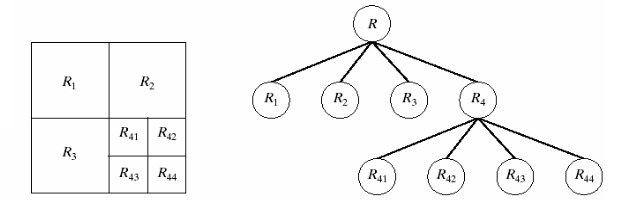
\includegraphics[width=3.5in]{tree3.png}
  \end{figure}
\end{frame}

\begin{comment}
\subsection{Region spliting and merging}
\begin{frame}
    \frametitle{Region spliting and merging}
   
    \textbf{Region splitting:}\\
        \begin{itemize}
        \item Region splitting starts with the whole image as a single region and subdivides it into subsidiary regions recursively while a condition of homogeneity is not satisfied.
        \end{itemize}
    \textbf{Region merging:}\\
        \begin{itemize}
        \item Region merging is the opposite of region splitting and works as a way of avoiding over-segmentation 
        \item It starts with small regions and merge the regions that have similar characteristics
        \end{itemize}
\end{frame}
\end{comment}

%\begin{frame}
%  \frametitle{Region Spliting and Merging}
%  \begin{figure}[!ht]
%  \centering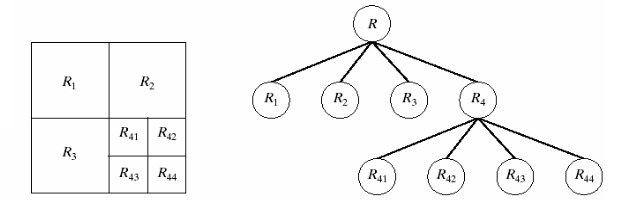
\includegraphics[width=4.0in]{tree3.png}
%  \end{figure} 
%\end{frame}

\begin{comment}
\begin{frame}
    \frametitle{Region split and merge}
    \begin{itemize}
    \item 对于任何区域Ri,如果P(Ri)=FALSE,就将每个区域都拆分为4个相连的象限区域
    \item 将P(Rj∪Rk)=TRUE的任意两个相邻区域Rj和Rk进行聚合
    \item 当再无法进行聚合或拆分时操作停止
    \end{itemize}
\end{frame}
\end{comment}

\begin{frame}
    \frametitle{Region Splitting and Merging}
    \begin{enumerate}[{\color{black}{\Large (B)}}]
    \item  \textbf{\Large Algorithm:}
    \end{enumerate}
  %  \textbf{\Large Algorithm:}\\
    \begin{itemize}
    \item[step1] {\emph{If}} a region $R$ is inhomogeneous ($P_1(R)=FALSE$), {\emph{then}} $R$ is split into four sub-regions.
    \item[step2] {\emph{If}} two adjacent regions $R_i$ and $R_j$ are homogeneous ($P_2(R_i \cup R_j)=TRUE$), {\emph{then}} they are  merged.
    \item[step3] The algorithm stops when no further splitting or merging is possible.
  \begin{figure}[!ht]
  \centering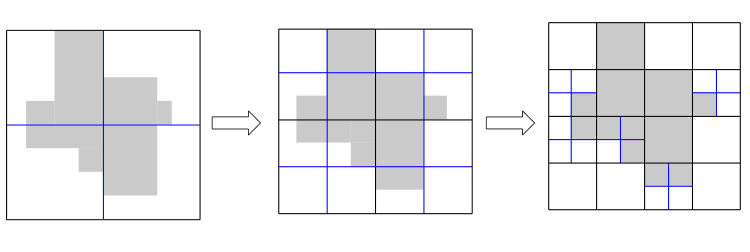
\includegraphics[width=3.5in]{split.png}
  \end{figure} 
    \end{itemize}
\end{frame}

\begin{frame}
  \frametitle{Region Splitting and Merging}
  \begin{figure}[!ht]
  \centering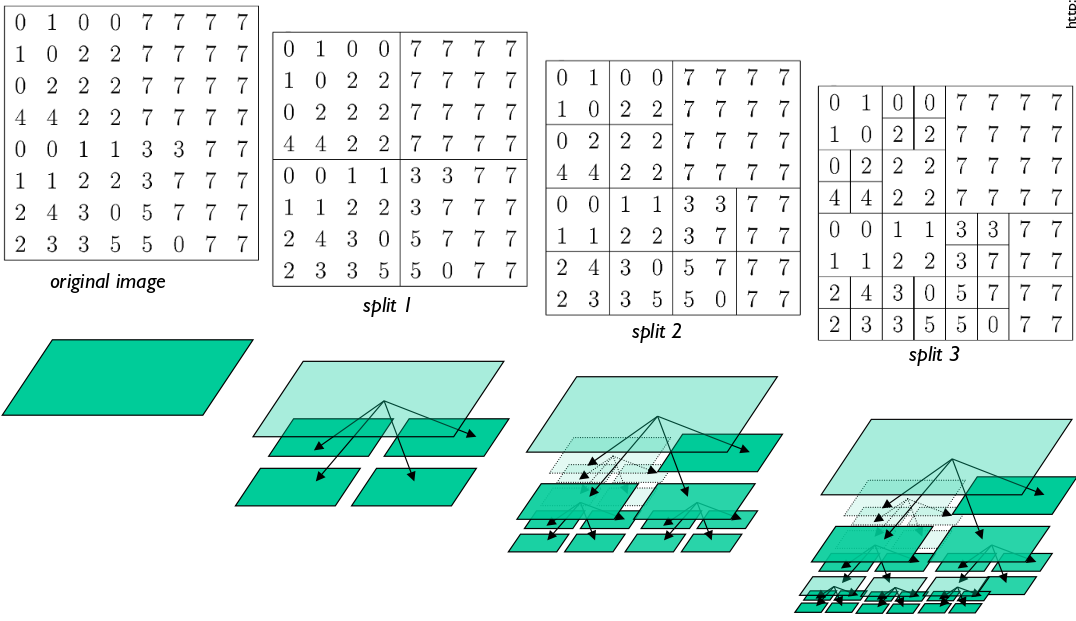
\includegraphics[width=3.5in]{tree2.png}
  \caption{$T$=1}
  \end{figure} 
\end{frame}

\begin{comment}
\begin{frame}
    \frametitle{Region split and merge}
    \begin{itemize}
    \item 思路直接,不依赖“种子点”的选择
    \item 像素级的分裂增加合并的工作量,提高时间复杂度
    \item 可能会使分割区域的边界破坏
    \end{itemize}
\end{frame}
\end{comment}



\begin{frame}
  \frametitle{Region Splitting and Merging}
  \begin{figure}[!ht]
  \centering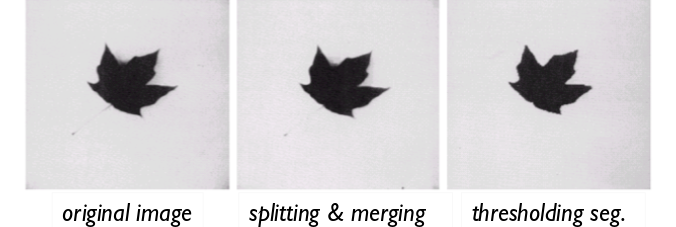
\includegraphics[width=3.5in]{region2.png}
  \end{figure} 
\end{frame}

\begin{frame}
    \frametitle{Region Splitting and Merging}
    \begin{enumerate}[{\color{black}{\Large (C)}}]
    \item  \textbf{\Large Advantages:}
    \end{enumerate}
%    \textbf{\Large Advantages:}\\
        \begin{itemize}
        %\item 
	\item Applicability in complex scenarios
    %    \item Simple conceptually
        \end{itemize}
    \begin{enumerate}[]
    \item  \hspace{0.25in}\textbf{\Large Disadvantages:}
    \end{enumerate}
 %   \textbf{\Large Disadvantages:}\\
        \begin{itemize}
        \item Cost of time and calculation
        \item Breaking boundaries of regions
    %    \item Dependent on seed point and pre-defined criteria
   %     \item Sensitive to noise
    \end{itemize}
\end{frame}

\begin{comment}
\begin{frame}
    \frametitle{Region split and merge}
    \begin{itemize}
    \item 
    \item The cost of time
    \end{itemize}
\end{frame}
\end{comment}

\subsection{Watershed}
\begin{frame}
    \frametitle{Watershed}
    \begin{enumerate}[{\color{black}{\Large (A)}}]
    \item  \textbf{\Large Idea:}
    \end{enumerate}
    \begin{itemize}
        \item[-] {\color{blue}{Hole}}: Image that a hole is done through each local minimum.\\ 
	\hspace{0.4in}The entire topography is flooded with water rising through the holes at a uniform rate.
        \item[-] {\color{blue}{Dam}}: When rising water in adjacent catchment basins is about the merge, a dam is built up to prevent merging.
        \item[-] {\color{blue}{Lines}}: These dam boundaries correspond to the watershed lines.
    \end{itemize}
  \begin{figure}[!ht]
  \centering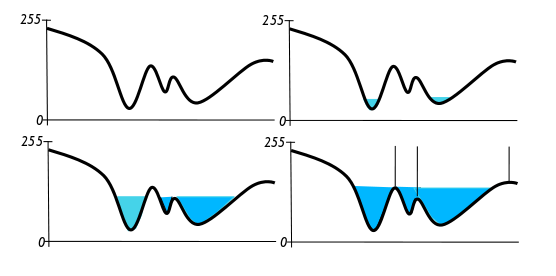
\includegraphics[width=2.5in]{region3.png}
  \end{figure} 
\end{frame}



%\begin{frame}
%  \frametitle{Watershed}
%%  \begin{figure}[!ht]
%  \centering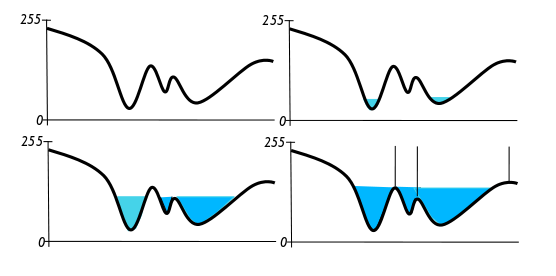
\includegraphics[width=3.5in]{region3.png}
%  \end{figure} 
%\end{frame}f


\begin{frame}
  \frametitle{Watershed}
  \begin{figure}[!ht]
  \begin{minipage}[t]{0.6\textwidth}
  \centering
  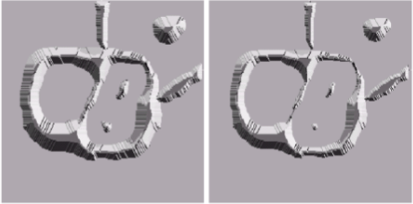
\includegraphics[width=2.5in]{region4.png}
  \end{minipage}
  \begin{minipage}[t]{0.6\textwidth}
  \centering
  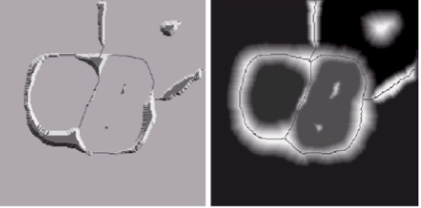
\includegraphics[width=2.5in]{region5.png}
  \end{minipage} 
  \end{figure}  
\end{frame}

\begin{frame}
    \frametitle{Watershed}
%    \textbf{Principle:}\\
%        \begin{itemize}
%        \item To prevent the merging of water from two catchment basins
%        \end{itemize}
    \begin{enumerate}[{\color{black}{\Large (B)}}]
    \item  \textbf{\Large Algorithm:}
    \end{enumerate}
%   \textbf{\Large Algorithm:}\\
        \begin{itemize}
        \item[step1] Start with all pixels with the {\textbf{lowest}} possible value. These pixels form the basis for initial watershed.
        \item[step2] For each group of pixels of intensity level $k:$ %($k$ means the difference between the neighboring pixels of regions and ):
	     \begin{itemize}
             \item[-] \emph{If} the pixels are adjacent to exactly {\textbf{one}} exising region, add these pixels to that region. 
             \item[-] \emph{Else if} the pixels are adjacent to {\textbf{more than one}} existing regions, mark boundary. 
	           \begin{itemize}
		   \item[-] \emph{Else} start a new region.
		   \end{itemize}
             \end{itemize}
  %      \item These dam boundaries correspond to the watershed lines
        \end{itemize}
\end{frame}


\begin{frame}
  \frametitle{Watershed}
  \begin{figure}[!ht]
  \begin{minipage}[t]{0.35\textwidth}
  \centering
  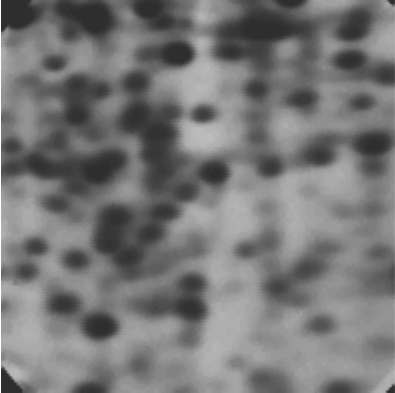
\includegraphics[width=1.5in]{water_origin.png}
  \end{minipage}
  \begin{minipage}[t]{0.35\textwidth}
  \centering
  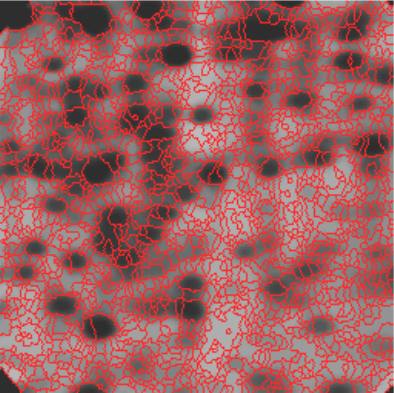
\includegraphics[width=1.5in]{water_over.png}
  \end{minipage} 
  \end{figure}  
\end{frame}
%\begin{frame}
%    \frametitle{Watershed}
  %  \textbf{Underlying operation:}\\
%	\begin{itemize}
  %       \item \textbf{Binary} morphological dilation 
 %       \end{itemize}
 %   \textbf{Dam construction sub-algorithm:}\\
%	\begin{itemize}
%	\item Initially, the set of pixels with minimum gray level are 1, others are 0
%	\item In each subsequent step, we flood the 3D topography from below and the pixels covered by the rising water are 1s and others 0s
%	\item At flooding step n-1, there are two connected components. At flooding step n, there is only one connected component
%	\end{itemize}
%	\end{frame}

\begin{comment}
\begin{frame}
    \frametitle{Watershed}
    \textbf{Problem:}\\
        \begin{itemize}
        \item Due to noise and other local irregularities of the gradient, over-segmentation may occur
        \end{itemize}
    \textbf{Solution:}\\
	\begin{itemize}
         \item Marker-controlled watershed segmentation
	      \begin{itemize}
	      \item Exclude a number of non-signfificant minima
	      \item The exclusion is done implicitly using markers on the blobs to specify the only allowed regional minima
	      \end{itemize}
        \end{itemize}
\end{frame}
\end{comment}

\begin{comment}
\begin{frame}
    \frametitle{Watershed}
    \begin{enumerate}[{\color{black}{\Large (C)}}]
    \item  \textbf{\Large Improved Algorithm:}
    \end{enumerate}
 %   \textbf{\Large Improved Algorithm:}\\
        \begin{itemize}
        \item Label each minimum with a distinct label. Initialize a queque $Q$ with the labeled nodes.
         \item Extract from $Q$ a node $x$ of minimal altitude $f$ or $f(x)=min \{ f(y) \mid y \subset S \} $
	 \item Attribute the label of $x$ to each non-labeled node $y$ adjacent to $x$, and insert $y$ in $S$
	 \item Repeat Step 2 and 3 until $S$ is empty
        \end{itemize}
\end{frame}
\end{comment}

\begin{frame}
    \frametitle{Watershed}
%    \textbf{Principle:}\\
%        \begin{itemize}
%        \item To prevent the merging of water from two catchment basins
%        \end{itemize}
    \begin{enumerate}[{\color{black}{\Large (C)}}]
    \item  \textbf{\Large Improved Algorithm:}
    \end{enumerate}
%   \textbf{\Large Algorithm:}\\
        \begin{itemize}
        \item[step1] Initially, {\textbf{label some pixels}} in your interested regions manually. \\
	Start with 8-neighborhood or 4-neighborhood of the labeled pixels. 
        \item[step2] For each group of pixels of intensity level $k$ ($k$ means the difference between marked pixels and the neighboring pixels) :
	     \begin{itemize}
             \item[-] \emph{If} the pixels are adjacent to exactly {\textbf{one}} exising region, add these pixels to that region. 
             \item[-] \emph{Else if} the pixels are adjacent to {\textbf{more than one}} existing regions, marks boundary. 
	        %   \begin{itemize}
		%   \item[-] \emph{Else} start a new region.
		%   \end{itemize}
             \end{itemize}
  %      \item These dam boundaries correspond to the watershed lines
        \end{itemize}
\end{frame}


\begin{frame}
  \frametitle{Watershed}
  \begin{figure}[!ht]
  \begin{minipage}[t]{0.4\textwidth}
  \centering
  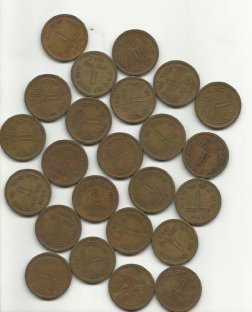
\includegraphics[width=1.5in]{watershed1.png}
  \end{minipage}
  \begin{minipage}[t]{0.4\textwidth}
  \centering
  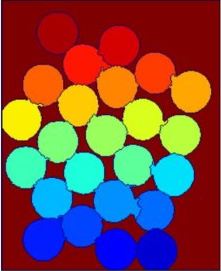
\includegraphics[width=1.5in]{watershed3.png}
  \end{minipage} 
  \end{figure}  
\end{frame}

\end{document}
